
\section{Experiments}

\begin{table*}[h]
\small
\centering
\caption{\textbf{Performance comparison of VideoITG integrated with different Video-LLMs, varying in both the size of the answering LLM and the number of sampled frames.}``UNI-$k$'' denotes UNIform sampling of $k$ frames, while ``ITG-$k$'' refers to selecting the Top $k$ frames based on relevance scores generated by our proposed VideoITG.
}
\vspace{-2mm}
\resizebox{\textwidth}{!}{
\begin{tabular}{ll|c|c|ccc|c|c}
\toprule
\multirow{2}{*}{\textbf{LMM}} & \multirow{2}{*}{\textbf{Selection}} & \multicolumn{1}{c|}{\textbf{LongVideoBench}} & \multicolumn{1}{c|}{\textbf{MLVU}} & \multicolumn{3}{c|}{\textbf{VideoMME}} & \multicolumn{1}{c|}{\textbf{CG-Bench-mini}} & \multirow{2}{*}{\textbf{Average}} \\
\cmidrule(lr){3-3} \cmidrule(lr){4-4} \cmidrule(lr){5-7} \cmidrule(lr){8-8} 
& & \textit{8min} & \textit{12min} & \textit{S (2 min)} & \textit{M (10 min)} & \textit{L (40 min)} & \textit{27min}  \\
\midrule
\multirow{2}{*}{InternVL2.5-8B} & UNI-32 & 58.3 & 66.4 & 75.1 & 61.7 & 53.1 & 37.7 & 58.7 \\
& ITG-32  & \cellcolor[HTML]{DAEFF9} \textbf{61.9} \textbf{(+3.6)} & \cellcolor[HTML]{DAEFF9} \textbf{75.0} \textbf{(+8.6)} & \cellcolor[HTML]{DAEFF9} \textbf{78.0} \textbf{(+2.9)} & \cellcolor[HTML]{DAEFF9} \textbf{67.1} \textbf{(+5.4)} & \cellcolor[HTML]{DAEFF9} \textbf{56.9} \textbf{(+3.8)} & \cellcolor[HTML]{DAEFF9} \textbf{46.7} \textbf{(+9.0)} & \cellcolor[HTML]{DAEFF9} \textbf{64.3} \textbf{(+5.6)} \\
\midrule
\multirow{2}{*}{InternVL2.5-26B} & UNI-32 & 55.6 & 71.3 & 78.1 & 67.1 & 56.9 & 40.6 & 61.6 \\
& ITG-32  & \cellcolor[HTML]{DAEFF9} \textbf{63.0} \textbf{(+7.4)} & \cellcolor[HTML]{DAEFF9} \textbf{78.9} \textbf{(+7.6)} & \cellcolor[HTML]{DAEFF9} \textbf{80.8} \textbf{(+2.7)} & \cellcolor[HTML]{DAEFF9} \textbf{69.0} \textbf{(+1.9)} & \cellcolor[HTML]{DAEFF9} \textbf{59.9} \textbf{(+3.0)} & \cellcolor[HTML]{DAEFF9} \textbf{48.7} \textbf{(+8.1)} & \cellcolor[HTML]{DAEFF9} \textbf{66.7} \textbf{(+5.1)} \\
\midrule
\multirow{2}{*}{InternVL3.5-8B} & UNI-32 & 60.0 & 70.0 & 77.0 & 62.4 & 53.4 & 40.9 & 60.6 \\
& ITG-32  & \cellcolor[HTML]{DAEFF9} \textbf{65.7} \textbf{(+5.7)} & \cellcolor[HTML]{DAEFF9} \textbf{74.1} \textbf{(+4.1)} & \cellcolor[HTML]{DAEFF9} \textbf{78.4} \textbf{(+1.4)} & \cellcolor[HTML]{DAEFF9} \textbf{65.9} \textbf{(+3.5)} & \cellcolor[HTML]{DAEFF9} \textbf{59.0} \textbf{(+5.6)} & \cellcolor[HTML]{DAEFF9} \textbf{47.6} \textbf{(+6.7)} & \cellcolor[HTML]{DAEFF9} \textbf{65.1} \textbf{(+4.5)} \\
\midrule
\multirow{2}{*}{Qwen3-VL} & UNI-32 & 59.1 & 64.1 & 76.0 & 60.9 & 55.1 & 40.1 & 59.2 \\
& ITG-32  & \cellcolor[HTML]{DAEFF9} \textbf{63.6} \textbf{(+4.5)} & \cellcolor[HTML]{DAEFF9} \textbf{77.2} \textbf{(+13.1)} & \cellcolor[HTML]{DAEFF9} \textbf{79.9} \textbf{(+3.9)} & \cellcolor[HTML]{DAEFF9} \textbf{66.6} \textbf{(+5.7)} & \cellcolor[HTML]{DAEFF9} \textbf{60.3} \textbf{(+5.2)} & \cellcolor[HTML]{DAEFF9} \textbf{47.3} \textbf{(+7.2)} & \cellcolor[HTML]{DAEFF9} \textbf{65.8} \textbf{(+6.6)} \\
\midrule
\multirow{2}{*}{LLaVA-Video-7B} & UNI-32 & 58.7 & 66.8 & 76.3 & 60.3 & 52.7 & 35.8 & 58.4 \\
& ITG-32  & \cellcolor[HTML]{DAEFF9} \textbf{61.6} \textbf{(+2.9)} & \cellcolor[HTML]{DAEFF9} \textbf{74.6} \textbf{(+7.8)} & \cellcolor[HTML]{DAEFF9} \textbf{77.3} \textbf{(+1.0)} & \cellcolor[HTML]{DAEFF9} \textbf{65.9} \textbf{(+5.6)} & \cellcolor[HTML]{DAEFF9} \textbf{55.2} \textbf{(+2.5)} & \cellcolor[HTML]{DAEFF9} \textbf{42.8} \textbf{(+7.0)} & \cellcolor[HTML]{DAEFF9} \textbf{62.9} \textbf{(+4.5)} \\
\midrule
\multirow{2}{*}{Eagle2.5-8B} & UNI-32 & 63.0 & 67.8 & 78.8 & 64.1 & 55.9 & 41.2 & 61.8 \\
& ITG-32  & \cellcolor[HTML]{DAEFF9} \textbf{66.8 (+3.8)} & \cellcolor[HTML]{DAEFF9} \textbf{76.5 (+8.7)} & \cellcolor[HTML]{DAEFF9} \textbf{80.0 (+1.2)} & \cellcolor[HTML]{DAEFF9} \textbf{67.8 (+3.7)} & \cellcolor[HTML]{DAEFF9} \textbf{60.3 (+4.4)} & \cellcolor[HTML]{DAEFF9} \textbf{49.0 (+7.8)} & 
\cellcolor[HTML]{DAEFF9} \textbf{66.7 (+4.9)} \\
\bottomrule
\end{tabular}}
\label{tab:video}
\vspace{-2mm}
\end{table*}


 % & UNI-64 & 65.2 & 72.7 & 80.0 & 65.9 & 58.4 & 44.5 & 61.8 \\

%  & UNI-64 & 59.9 & 70.2 & 75.8 & 63.0 & 54.7 & 36.9 & 60.1 \\
% & ITG-64  & \cellcolor[HTML]{DAEFF9} \textbf{60.9} \textbf{(+1.0)} & \cellcolor[HTML]{DAEFF9} \textbf{76.3} \textbf{(+6.1)} & \cellcolor[HTML]{DAEFF9} \textbf{76.1} \textbf{(+0.3)} & \cellcolor[HTML]{DAEFF9} \textbf{66.0} \textbf{(+3.0)} & \cellcolor[HTML]{DAEFF9} \textbf{57.0} \textbf{(+2.3)} & \cellcolor[HTML]{DAEFF9} \textbf{42.9} \textbf{(+6.0)} & \cellcolor[HTML]{DAEFF9} \textbf{63.2} \textbf{(+3.1)} \\

\begin{table*}[!h]
\centering
\caption{\textbf{Empirical studies on the VideoITG-40k dataset and VideoITG model design.} We adopt Variant-C for subsequent experiments. ``No Images" and ``No Videos" indicate that image-text data (LAION-CC-SBU-558K \& LLaVA-OV-SI) or video data (LLaVA-Video-178K) are excluded from pre-training, respectively.}
\vspace{-2mm}
\resizebox{\textwidth}{!}{%
\setlength{\tabcolsep}{8pt}
\begin{tabular}{l|c|ccc|c|c|c}
\toprule
\multirow{2}{*}{\textbf{Abaltion}} &
\multirow{2}{*}{\textbf{Experiment}} &
\multicolumn{3}{c|}{\textbf{Videomme}} &
\multicolumn{1}{c|}{\textbf{MLVU}} &
\multicolumn{1}{c|}{\textbf{LongVideoBench}} &
\multicolumn{1}{c}{\textbf{Average}} \\

&& \textbf{Short} (\%) $\uparrow$ & \textbf{Medium} (\%) $\uparrow$ & \textbf{Long} (\%) $\uparrow$ & \textbf(\%) $\uparrow$ & \textbf(\%) $\uparrow$\\
\midrule

& Variant-A-7B & 51.0 & 44.8 & 44.4 & 45.7 & 56.8 & 48.5 \\
\textbf{Architecture}
& Variant-B-7B & 77.9 & 66.0 & 56.2 & 74.6 & 61.3 & 67.2 \\
\textbf{Design} & \cellcolor[HTML]{DAEFF9}Variant-C-7B &\cellcolor[HTML]{DAEFF9}\textbf{78.0} &\cellcolor[HTML]{DAEFF9}\textbf{67.1} & \cellcolor[HTML]{DAEFF9}56.9 & \cellcolor[HTML]{DAEFF9}\textbf{75.0} & \cellcolor[HTML]{DAEFF9}\textbf{61.9} & \cellcolor[HTML]{DAEFF9}\textbf{67.8} \\
& Variant-C-3B & 77.1 & 64.8 & 56.0 & 74.5 & 61.5 & 66.8\\
\midrule 
\textbf{Dataset}& No Clip Captioning & 77.5 & 63.1 & 53.4 & 73.2 & 61.7 &  65.8  \\
\textbf{Construction} & No Frame Localization & 77.6 & 65.8  & 56.8 & 74.1 & 61.5 & 67.2 \\
\midrule 
\textbf{Pre-training}& No Videos & 77.2 & 64.9 & \textbf{57.4} & 74.5 & 61.6 & 67.1 \\
\textbf{Data} & No Images \& Videos & 76.6 & 63.0  & 54.4 & 69.1 & 58.6 & 64.3 \\
\bottomrule
\end{tabular}}
\vspace{-2mm}
\label{ablation_table_models}
\end{table*}


\subsection{Implementation details}
We follow the training approach of LLaVA-Video~\cite{zhang2024video}, using the pretrained model as the initialization for our VideoITG model's pre-training. We employ SigLIP~\cite{zhai2023sigmoid} as the vision encoder and Qwen2~\cite{wang2024qwen2} as the language model. Initially, we train the MLP projector on image caption datasets with a batch size of 256 and a learning rate of \(1 \times 10^{-3}\). Then, we fine-tune all model parameters on the LLaVA-OV-SI~\cite{li2024llavaonevision} and LLaVA-Video datasets. During this stage, the video frame sampling rate is set to 64, and the LLM's maximum sequence length is set to 16K. We then train the VideoITG model on the proposed VideoITG-40K dataset, adjusting the video sampling rate to 1 fps. 

Throughout training and inference, we employ a dynamic token spatial size strategy~\cite{liu2025oryx}. Across all stages, the LLM's learning rate is \(2 \times 10^{-5}\), and in the final stage, the learning rate for the classification head is \(2 \times 10^{-4}\). To fairly compare with other leading video LMMs, we primarily use results from their original papers. When results are unavailable, we integrate the models into LMMs-Eval~\cite{zhang2024lmms} and assess them under consistent settings. Due to context length constraints, we support up to 512 video frames as input (with 16 visual tokens per frame) for the VideoITG model, from which we select the top 32 frames based on their scores by default. 

\subsection{Main results}



\noindent \textbf{Comparisons with other frame selection methods.}
As shown in Table~\ref{tab:main_comparisons}, our proposed VideoITG demonstrates \textbf{\textit{three notable advantages}} over existing selection strategies: 

\textbf{(i) Consistant Improvement}: VideoITG consistently outperforms Uniform sampling across all benchmarks and model settings. It achieves an average gain of \textbf{+6.7} (54.9$\rightarrow$61.6) on LLaVA-OneVision-7B and \textbf{+6.2} (54.1$\rightarrow$60.3) on Qwen2-VL, with similar trends on LLaVA-Video-7B (+2$\sim$3 points). These steady improvements across diverse models and datasets highlight the \textbf{robustness} and \textbf{general applicability} of our frame selection strategy in enhancing video understanding under challenging scenarios.

\textbf{(ii) Precision in Selection}: When using LLaVA-Video as baseline, VideoITG achieves superior accuracy using only 32 selected frames, outperforming other methods that use \textbf{more frames} (\textit{e.g.}, 50-64) on MLVU and VideoMME, highlighting the effectiveness of our strategy in identifying the most informative frames. As shown in Figure~\ref{fig:frames}, our VideoITG method achieves comparable performance to uniform sampling with 64 frames using only 16 frames on VideoMME, and also outperforms other methods with 32 frames, highlighting the precision of our frame selection strategy. 

\textbf{(iii) Robust Performance:} Compared to training-based methods such as Q-Frame and Frame-Voyager, VideoITG achieves more substantial improvements across three long video understanding benchmarks. For instance, it boosts the average score from 59.5 (Frame-Voyager) and 57.6 (Q-Frame) to \textbf{61.6} and \textbf{60.3} under the same settings. These consistent gains highlight the strong adaptability of VideoITG across diverse scenarios.

We find that on LongVideoBench, increasing frames has limited impact, likely because many tasks are text referring. Our VideoITG also samples at lower resolution, indicating room for finer-grained content recognition.
 
\vspace{1mm}
\noindent\textbf{Results on newer backbone (Qwen3-VL).}
To verify that our gains are not tied to a specific backbone generation, we evaluate VideoITG on the newer Qwen3-VL model. The results are included in Table~\ref{tab:video}, showing consistent improvements over the UNI-32 baseline across LongVideoBench, MLVU, VideoMME (S/M/L), and CG-Bench-mini.




\noindent\textbf{Extension to more Video-LLMs.} Extending our VideoITG on diverse Video-LLMs with difeerent model scales further presents its \textbf{\textit{two compiling advantages}}: 

\textbf{(i) Model Size Scalability}:
Table~\ref{tab:video} demonstrates that integrating VideoITG with Video-LLMs of different sizes consistently yields substantial performance improvements over uniform sampling. For example, on InternVL2.5-8B, VideoITG improves the average score from $58.7\%$ to $64.3\%$ ($+5.6$), while on the larger InternVL2.5-26B, the improvement is from $61.6\%$ to $66.7\%$ ($+5.1$). Notably, InternVL2.5-8B with VideoITG even surpasses the InternVL2.5-26B baseline on both average score ($64.3\%$ vs. $61.6\%$) and long-video benchmarks such as CG-Bench ($46.7\%$ vs. $40.6\%$), indicating that effective frame selection can provide greater gains than simply increasing model size. 

\begin{figure*}[!h]
\centering
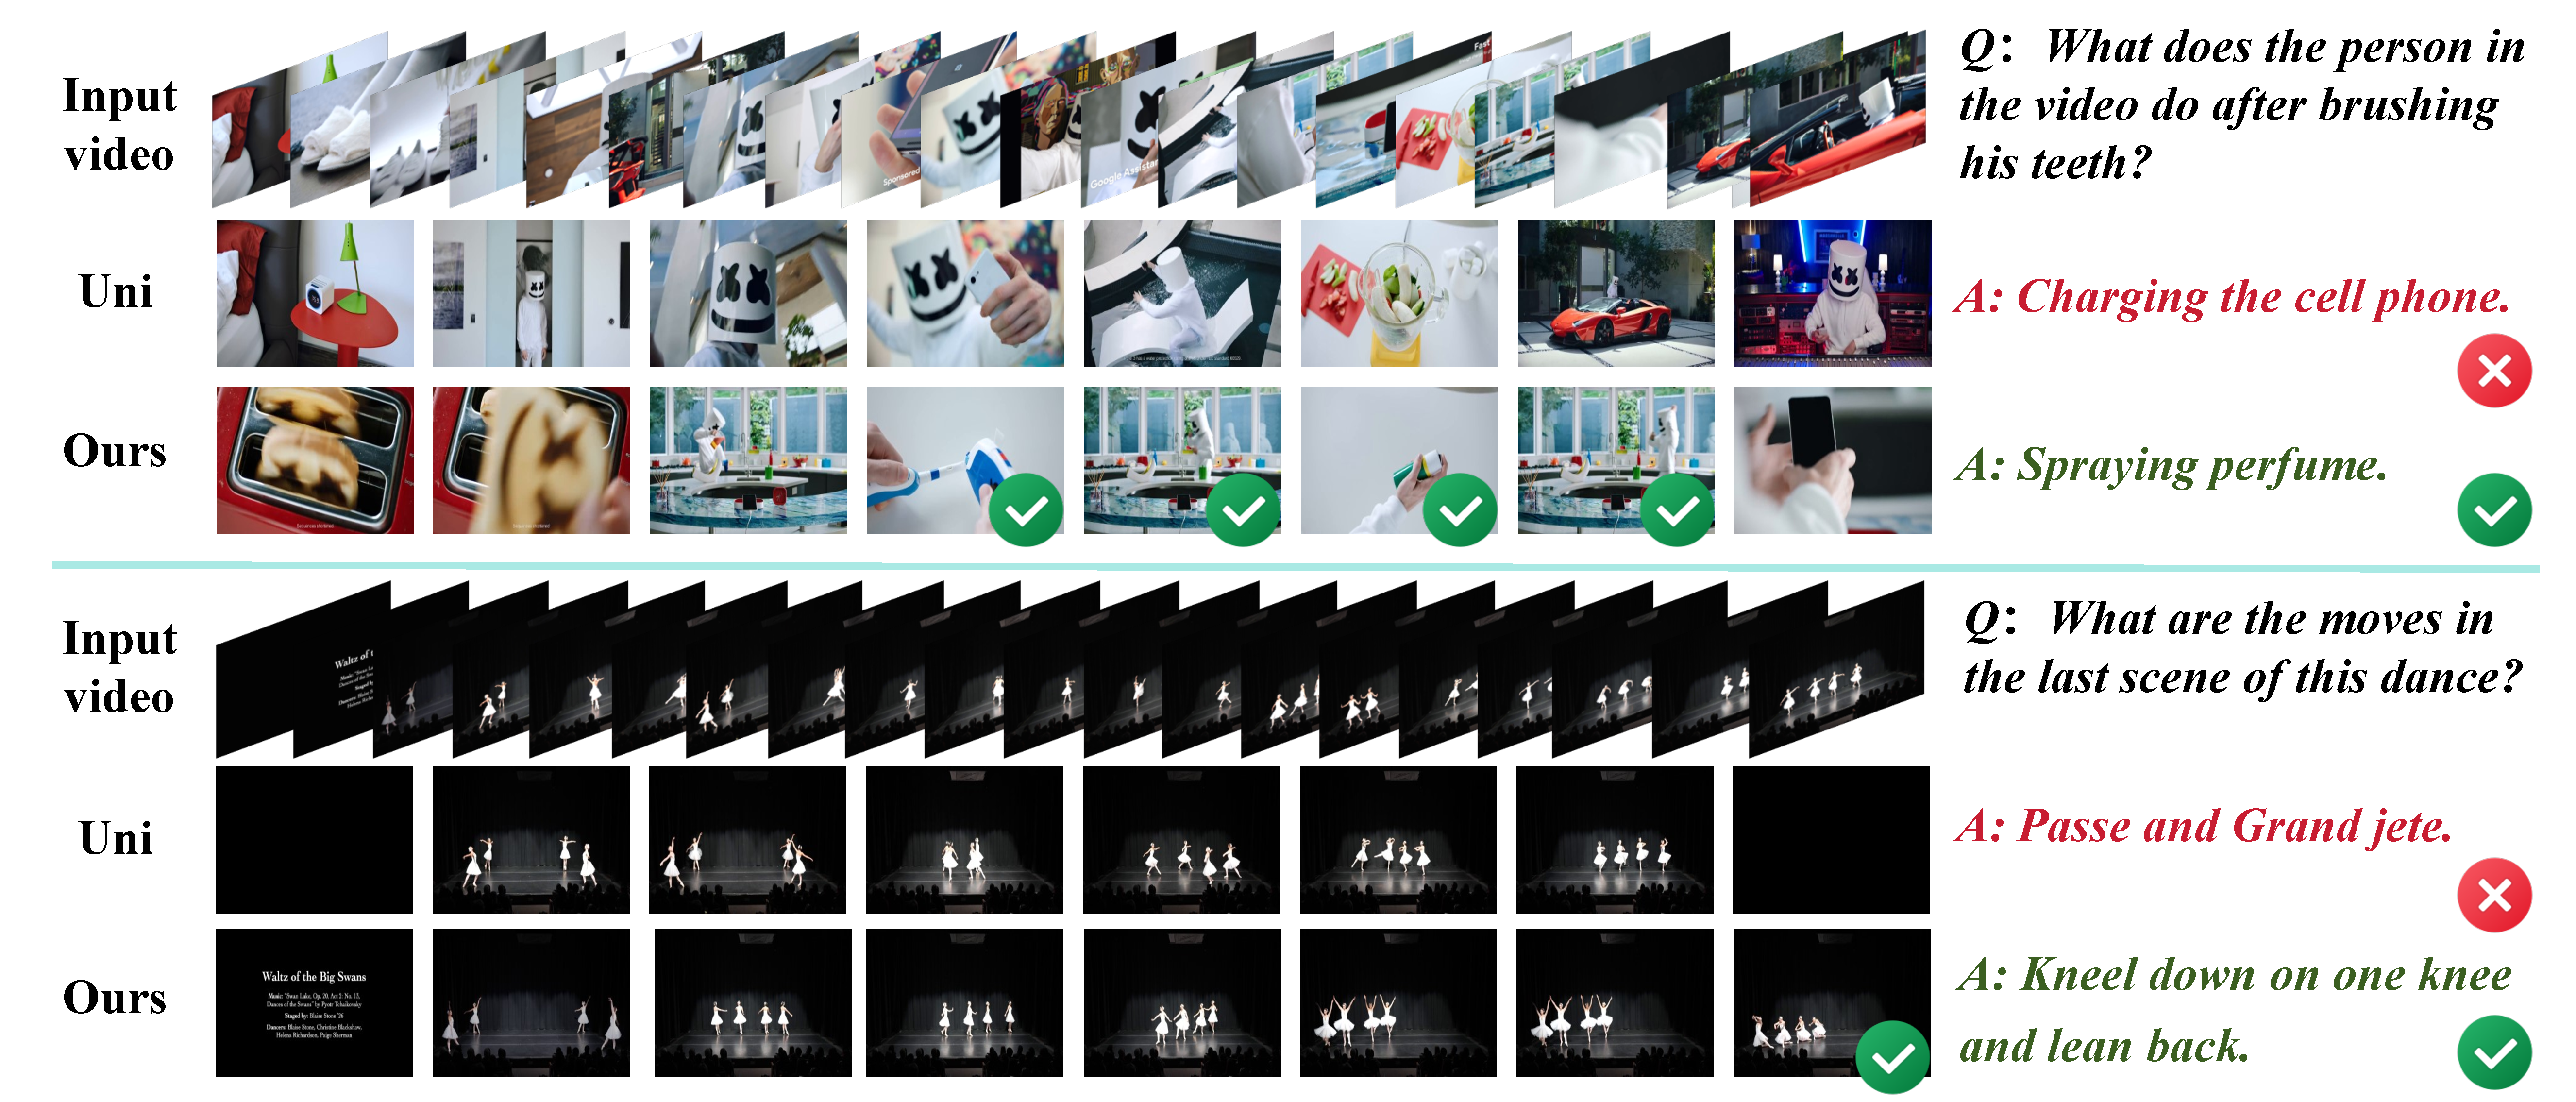
\includegraphics[width=\linewidth]{vis.pdf}
\vspace{-7mm}
\caption{\textbf{Two examples of how different sampling strategies impact video understanding.} We mark the identified key frames that directly answer the question with green check-marks.}
\label{vis}
\end{figure*}

(ii) \textbf{Model Diversity Adaptability}:
We further evaluate VideoITG across diverse Video-LLMs, each trained on different data distributions and objectives. The results show that VideoITG consistently outperforms uniform sampling for all models and benchmarks. For instance, on LLaVA-Video-7B, VideoITG raises the average score by $4.5$ \% ($62.9\%$ vs. $58.4\%$), and on Eagle2.5-8B, the improvement reaches $4.9$ points ($66.7\%$ vs. $61.8\%$). These consistent gains across models with varying architectures and training data highlight the strong adaptability and robustness of our method.

\subsection{Ablation on VideoITG design choices}
Table~\ref{ablation_table_models} presents a comprehensive analysis on the design of VideoITG, directly supporting our key contributions.



\noindent\textbf{Architecture Design.} 
First, we compare the three variants of our model architecture in Fig.~\ref{fig:model}. We observe that Variant A, which is based on the text generation paradigm, performs the worst. One possible reason is that text generation models trained with the next-token prediction paradigm suffer from sparse supervision due to teacher forcing, where previous frame selections influence subsequent ones, making the training process less efficient compared to discriminative classification models. We find that Variant C with full-attention outperforms Variant B with causal attention. This improvement may be attributed to full-attention's larger receptive field, which enables global temporal relationship modeling and allows all tokens to access the textual query. Moreover, model scale yields a consistent but modest gain: the 7B model surpasses the 3B counterpart across all benchmarks, raising the overall average from 66.8\% to 67.8\%.



\noindent\textbf{Dataset Construction.} We analyze our data annotation strategies to demonstrate the effectiveness of our pipeline. Ablation studies show that the performance degrades when Instructed Clip Captioning are removed (using a VLM to directly select temporal boundaries based on visual inputs), with accuracy dropping from 56.9\% to 53.4\% on Videomme Long videos and from 75.0\% to 73.2\% on MLVU. This demonstrates that ensuring information diversity is crucial for maintaining comprehensive feature  representation of videos. Similarly, removing Instructed Frame Localization (learning all frame index within corase temporal boundaries using VideoITG Model) decreases performance, particularly on Videomme Medium videos (from 67.1\% to 65.8\%). These results confirm that both stages are essential for optimal model performance and validate our data construction approach of the VideoITG-40K dataset.

\noindent\textbf{Pre-training Data.} Finally, we investigate the impact of vision-language alignment pre-training on model performance. Our experiments reveal that removing video pre-training causes modest performance changes across benchmarks. This suggests that the benefits of video data for instructed temporal grounding tasks primarily stem from effective visual context length, yet this impact is relatively minor compared to vision-language alignment. This observation is further validated if we eliminate both image and video pre-training data, starting from a text-only large language model, where performance drops dramatically, with accuracy decreasing from 75.0\% to 69.1\% on MLVU and from 61.9\% to 58.6\% on LongVideoBench. This substantial degradation underscores that robust vision-language alignment is crucial to effective VideoITG training.%, as the model struggles to establish meaningful connections between visual content and textual instructions without this foundational knowledge.




\subsection{Visualization}
In Fig.~\ref{vis}, we compare uniform sampling and VideoITG sampling of 8 frames from the VideoMME~\cite{fu2024videomme} Benchmark. In the first case, VideoITG captures both brushing teeth and spraying perfume actions, enabling correct temporal ordering, while uniform sampling misses key cues. In the second case, VideoITG accurately captures rapid consecutive movements at the end, whereas uniform sampling fails to do so, leading to incomplete video understanding.


